\documentclass{VUMIFPSkursinis}
\usepackage{algorithmicx}
\usepackage{algorithm}
\usepackage{algpseudocode}
\usepackage{amsfonts}
\usepackage{amsmath}
\usepackage{bm}
\usepackage{caption}
\usepackage{color}
\usepackage{float}
\usepackage{graphicx}
\usepackage{listings}
\usepackage{subfig}
\usepackage{wrapfig}


% Titulinio aprašas
\university{Vilniaus universitetas}
\faculty{Matematikos ir informatikos fakultetas}
\department{Programų sistemų katedra}
\papertype{Kursinis darbas}
\title{Mobiliųjų programų testavimas remiantis TMMi modeliu.}
\titleineng{TMMi model based mobile application testing.}
\status{3 kurso 4 grupės studentas}
\author{Ričardas Mikelionis}
\supervisor{Lekt. dr. Vytautas Valaitis}
\date{Vilnius – \the\year}

% Nustatymai
\setmainfont{Palemonas}   % Pakeisti teksto šriftą į Palemonas (turi būti įdiegtas sistemoje)
\bibliography{bibliografija}

\begin{document}
\maketitle

\cleardoublepage
\pagenumbering{gobble}
\tableofcontents
\cleardoublepage
\pagenumbering{arabic}

\sectionnonum{Įvadas}
Nuo 2007, kai buvo pristatytas pirmasis iPhone jau praėjo kiek daugiau nei dešimt metų. Šio mobiliojo įrenginio, išmaniojo telefono (angl. Smartphone), pristatymas sukrėtė ir iš esmės pakeitė mobiliųjų kompiuterių rinką. Iki tol asmeniniai skaitmeniai asistentai (angl. PDA personal digital asistant) buvo nei prieinami, nei labai naudingi įprastam vartotojui, todėl juos turėjo keletas verslo pasaulio žmonių, o paprastas vartotojas su savimi nešiojosi krūvą skirtingą funkcionalumą atliekančių prietaisų: MP3 grotuvų, Fotoaparatų, nešiojamųjų kompiuterių, telefonų. iPhone žadėjo delne telpantį kompiuterį kiekvienam už prieinamą kainą, ir savo pažadą įvykdė. Vienas po kito ėmė rastis  mobiliosios operacinės sistemos, turėjusios tiesiogiai konkuruoti su iPhone naudojama iOS,  kaip PalmOS, Symbian, Windows 7 mobile, vėliau tapusi 8 ir 8.1 bei Android. Mobiliųjų kompiuterių bei telefonų rinką apėmė ir užplūdo krūvos prieinamų įrenginių, kurie su kiekviena nauja laida savo skaičiavimo sugebėjimais artėja arčiau ir arčiau to ką gali atlikti staliniai kompiuteriai, ir iš pažiūros 2017 metų išmanusis įrenginys savo specifikacijomis „ant popieriaus“ jau seniai pranoko 2007 metų kompiuterį.

Nors šiandien iš gausaus operacinių sistemų pasirinkimo rinkoje iš esmės išlikę tik dvi: iOS ir Android, tačiau  išmaniųjų prietaisų populiarumas toli gražu neblėsta. 2016 metais pasaulyje jau buvo apie 2.1 mlrd. išmaniųjų telefonų naudotojų, o iki 2020 planuojama, jog šis skaičius sieks 2.87 mlrd.\cite {statista.com}. Esant didžulei įrenginių paklausai proporcingai kyla poreikis ir programinei įrangai pritaikytai šiems įrenginiams - mobiliosioms programoms.

Šio darbu siekiama pateikti esminius skirtumus tarp įprastų darbastalio (angl. desktop) bei internetinių (angl. Web) programų ir mobiliųjų programų skirtų išmaniesiems įrenginiams kokybės užtikrinimo. Šio darbo tikslas - išanalizavus dabartinės rinkos mobiliųjų programų kūrimo procesų tendencijas, išskirti problemines mobiliųjų programų kokybės užtikrinimo sritis bei pateikti keletą probleminių sričių kokybės užtikrinimo sprendimų remiantis testų brandos modeliu.



\section{Mobiliųjų programų kokybės užtikrinimas.}

2013 metais atliktas tyrimas \cite {compuware.com} rodo, jog 79\% išmaniųjų telefonų naudotojų išbando atsisiųstą programėlę tik kartą prieš ištrindami. Didelė to priežastis yra žemesnė mobiliųjų programų kokybė palyginus su tuo ką vartotojai yra įpratę matyti savo naršyklėse, ar darbastalio programose. Išmaniųjų telefonų naudotojai yra pratę prie nemokamos ar žymiai mažiau kainuojančios programinės įrangos, kuri gauna nuolatinius atnaujinimus. (Pvz.: Adobe photoshop express iOS 0eur., Adobe Photoshop Windows 10 290eur./m. \cite{adobe.com}). Kyla kainų dilema: norint palaikyti žemas kainas rinkoje reikia mažinti kainas ir kūrimo procese. Tai dažnai daroma taupant laiką, kur ir nukenčia kokybės užtikrinimo procesai.

Į mobiliųjų programų kūrimą vis dar žiūrima taip pat, kaip į interneto programų (angl. WEB application) ar darbastalio programų kūrimą, neįžvelgiant esminių skirtumų tarp šių dviejų programinės įrangos kūrimo procesų. Didžiulė įrenginių variacijų gausa, ir iš esmės išsiskiriantys naudojimosi mobiliąja programine įranga įpročiai turėtų versti kūrėjus į mobiliųjų programų kūrimą žvelgti kitaip.

\subsection{Mobiliųjų programų kūrimo proceso probleminės sritys.}
M. Satyanarayanan dar 1996-aisiais savo straipsnyje apie mobiliuosius kompiuterius puikiai aibrėžė esmines sritis, kurios išskiria mobiliuosius įrenginius nuo stacionariųjų. Išskirtos keturios sritys: riboti skaičiavimo ištekliai (angl. limited computing resources), apsauga ir pažeidžiamumas, galia (angl. performance) ir patikimumas bei riboti energijos ištekliai. \cite{Satyanarayanan:1996:FCM:248052.248053}

Iš esmės mobiliosios programos yra tokia programinė įranga, kuri veikia nešiojamame (mobiliame) įrenginyje. Tačiau į mobiliąją kompiuteriją žvelgiant per išmaniųjų telefonų prizmę mobiliųjų programų apibrėžimą galime sukonkretinti. Mobilioji programa (angl. mobile app) - programa suprojektuota veikti išmaniąjame telefone, planšetiniame kompiuteryje ar kitame mobiliame įrenginyje ir/arba, kaip įvestį, priimanti situacija paremtą (angl. context based) informaciją pvz. GPS signalas. \cite{6496451} Situacijos supratimas, naujimasis situacine informacija ir gabėjimas keisti savo veikimą yra dar vienas esminis mobiliųjų programų, ypač skirtų išmaniesiems telefonams, skiriamasis bruožas.

Remiantis šiais keturiais techniniais išskirtinumo bruožais, ir esminiu veikimo skirtumu galima pradėti išskirti problemines kokybės užtikrinimo sritis mobiliųjų programų kūrime. Laikant progamas išmaniesiems telefonams tyrimo baziniu objektu išskiriamos šios sritys:
\begin{itemize}
  \item  Ryšio sujungiamumo
  \item Ribotų išteklių
  \item Draugiškumo vartotojui
  \item Situacinio prisitaikymo
  \item Įrenginių gausos
  \item Naujų operacinių sistemų versijų
  \item Liečiamųjų ekranų
\end{itemize}

\subsubsection{Ryšio sujungiamumo probleminė sritis}
Sugebėjimas prisijungti prie mobiliojo ryšio stočių bei bevielio interneto taškų dažnai mobiliajai programai yra kritinis reikalavimas, be kurio ši nesugebės funcionuoti. Problema kyla dėl ryšio nepastovumo keliaujant. Keliaujant didelius atstumus vyksta persijungimai tarp mobilaus ryšio stotelių, vartotojas gali pakliūti į neryšio zoną, ar vietą kurioje veikia viso labo GPRS ar EDGE ryšys. Taip pat ir su bevielio interneto stotelėsmis, kurių dažna veikia vos 100m. spinduliu nesant jokiems trukdžiams. 

Testuojant šioje srityje derėtų atsižvelgti į jau egzistuojančius ryšio defektus esančius specifiniame testavimui naudojamame įrenginyje, ar operacinėje sistemoje. \cite{android_bugs} Testuojant programas kurios smarkiai remiasi į įrenginio sugebėjimą prisijungti prie interneto ar mobiliojo ryšio tinklų atsiranda poreikis atlikti funkcinius testus įvairuose ryšio sujungiamumo scenarijuose. Pagrindinis siekis yra užtikrinti teisingą programos veikimą, net dingus ryšiui ar šiam staiga smarkiai sulėtėjus.

\subsubsection{Ribotų išteklių probleminė sritis}
Kol mobilieji įrenginiai tampa vis galinesni ir galingesni, jie vis dar negali pasivyti satcionariųjų bei nešiojamųjų kompiuterių. Pavyzdžiui vienas iš galingesnių šiuo metu rinkoje esančių telefonų, Samsung Galaxy s8+ turi 6GB atminties bei 8 branduolių, palaikančių 8 gijas, sistemą mikroschemoje (angl. system on a chip) į kurią integruoti vaizdo procesorius bei pagrindinis procesoriai. \cite{samsung_s8} Šiuo metu didžioji dauguma vartotojams prieinamų motininių plokščių kompiuteriams palaiko iki 64GB atminties, o intel neseniai atskleidė savo naujosios kartos i9 procesorių liniją, kur aukščiausios klasės procesorius sudarytas iš 18 branduolių bei 36 gijų. \cite{intel_i9}

Testuojant šioje srityje būtina atsižvelgti į išteklių įrenginyje naudojimą paleidžiant bei naudojant programą. Tai daroma siekiant išvengti staigių našumo sumažėjimų, neteisingo, nenumatyto programos ar įrenginio veikimo staiga imant naudoti 100\% prieinamų išteklių. Pagrindinis testavimo siekis užtikrinti teisingą programos bei įrenginio veikimą esant skaičiavimo išteklių trūkumui.

\subsubsection{Draugiškumo vartotojui probleminė sritis}
Kūrėjai kuriantys programas mobiliosioms operacinėms sistemos (Android, iOS) privalo sekti operacinių sistemų kūrėjo nusatytas varotojų sąsajos gaires. Dėl įrenginių gausos, skirtingų dydžių bei raiškos ekranų atsiranda grafinių neatitikimų tikimybė. 

Testuojant šioje srityje būtina testavimą atlikti ant daug skirtingų įrenginių, veikiančių su skirtingomis operacinės sistemos versijomis bei skirtingų raiškų bei dydžių ekranais.

\subsubsection{Situacinio prisitaikymo probleminė sritis}
Didelė dalis mobiliųjų programų remiasi duomenimis gautais priklausomai nuo situacijos, iš įvairių sensorių išmaniajame įrenginyje. Dažnai išmanieji įrenginiai turi įvairių sensorių, kaip, mikrofonai, šviesos jutikliai, akselerometrai bei giroskopai, vaizdo kameros. Tokie įrenginiai turi ir keletą būdų komunikuoti, susijunti su kitais prietaisais, internetu: bluetooth, wifi, 4G/LTE, NFC. Visi šie sensoriai gali suteikti prigramai krūvą informacijos realiu laiku, atsižvelgiant į tai ką vartotojas veikia su įrenginiu, ar kur jis tuo metu yra.

Testuojant šioje srityje patikrinti visų įrenginių ir įvesčių kombinacijų praktiškai neįmanoma. Todėl testus reikia skirstyti į kontekstinius (angl. context-specific), bei nusistatyti užtektinus testų padengtumo kriterijus. Kuriant kontekstu paremtus testus, bei renkantis įrenginius su kuriais bus vykdomi testavimo atvejai verta atsižvelgti į konkrečiam įrenginiui būdingus ar operacinės sistemos versijai būdingus defektus. \cite{android_bugs}

\subsubsection{Įrenginių gausos probleminė sritis}
Rinkoje, vartotojams prieinami šimtai skirtingų mobiliųjų įrenginių iš skirtingų gamintojų, veikiančių su skirtingomis operacinėmis sistemomis, surinktų iš skirtingų komponentų. 2013 metais atlikto tyrimo metu buvo suskaičiuota, jog rinkoje yra apie 1800 unikalių vien Android operacine sistema paremtų įrenginių modelių. \cite{Muccini:2012:STM:2663608.2663615}

Testuojant šioje srityje reikia stengtis maksimizuoti testų padengtumą minimizuojant naudojamų įrenginių kiekį. Tą galima daryti grupuojant įrenginius, ir testuojant ne konkrečiuose įrenginiuose (mažiau įrenginių) tačiau grupėse. Pavyzdžiui:

Pirmoji grupė, žemiausio prioriteto testai, silpni, palyginus su dabartiniais pagrindinių gamintojų flagmanais, turintys silpnesnius procesorius, mažiau atminties, žemesnės raiškos ekranus. Paremti senesne operacinės sistemos versija, veikiantys su senesne naršykle. Dar vis populiarūs, tačiau gamintojo jau nebepalaikomi įrenginiai.

Antroji grupė, vidutinio prioriteto testai, vidutinio galingumo įrenginiai, dažniausiai kelių iteracijų, palyginius su dabartiniais pagrindinių išmaniųjų įrenginių gamintojų flagmanais, senumo pvz: iPhone 5s palyginus su iPhone 7. Jau gan seni, 3-2 metai, tačiau dar vis gamintojo palaikomi įrenginiai.

Trečioji grupė, patys naujausi <1 metų senumo įrenginiai. Paremti naujausia operacinės sistemos versija, naujausios kartos komponentais, turintys daugiau atminties, aukštesnės raiškos ekranus, nei praeitos iteracijos modeliai.\cite{6496451}

Testuojant pasirinkta įrenginių kombinacija įgalina keletą pasirinkimų, kaip tokį testavimą galima vykdyti: rankinis testavimas arba automatinis testavimas, komandos įmonėje arba žmonės pasamdyti iš kitų įmonių, testavimas pagal planą arba tiriamasis testavimas (angl. exploratory testing) bei emuliatorių, virtualių mašinų naudojimas arba testavimas ant realių, fizinių įrenginių

\subsubsection{Naujų operacinių sistemų probleminė sritis}
Mobiliosios operacinės sistemos, palyginus su operacinėmis sistemomis stacionariesiems kompiuteriams, yra išleidžiamos labai dažnai. Pastaruoju metu tiek iOS tiek Android nauja „numeruotoji“ versija yra išleidžiama kas met. Taip dažnai išleidžiant naują operacinės sistemos iteraciją gali kilti daugybė nesuderinamumo defektų, turint omenyje tai, kad ne visos versijos yra palaikomos, t.y. naujesnės programų versijos gali veikti tik su keliomis paskutinėmis operacinės sistemos iteracijomis.

Testuojant programas reikėtų atsižvelgti į egzistuojančius konkrečios operacinės sistemos versijos defektus, bei testuoti naudojant keletą skirtingų tos pat operacinės sistemos iteracijų. Taip siekiant įsitiktinti, ar defektai atsiradę mobiliojoje programoje buvo sukelti operacinės sistemos defekto, ar blogo kodo.

\subsubsection{Liečiamųjų ekranų probleminė sritis}
Liečiamieji ekranai yra pagrindinis, ir dažniausiai vienintelis įvesties pateikimo būdas mobiliuosiuose įrenginiuose. Dažna problema, ypač senesniuose įrenginiuose, yra lėtas prisilietimo prie ekrano atsakas, ar ekrano įvesties atsako laiko padidėjimas imant naudotis sudėtingesnėmis programomis.

Testuojant reikėtų naudoti daug skirtingų įrenginių, kurie iš esmės skiriasi savo specifikacijomis, ypač ekranų dydžiu, raiška. Pagrindinis testavimo objektas yra resursų pasiskirstymas. Tikrinama ar testuojama programinė įranga mobilajame įrenginyje „neryja“ resursų. Reikėtų stengtis įvykdyti didelės apkrovos scenarijų, kai programinė įranga veikia pilnu pajėgumu atlikdama didžiausių skaičiavimų reikalaujančias užduotis, ir tikrinti mobiliojo įrenginio atsako laiką.

\subsection{Integracinis testų brandos modelis - TMMi}
Testų brandos modelis buvo sukurtas, tam, kad įvairios organizacijos galėtų įvertinti bei įvertinę pagerinti savo testavimo procesus. Tai taip pat teikia naudą, kaip modelis, tiesiogine to žodžio prasme, kuris nurodo, kaip testavimo procesas turėtų  palaipsniui gerėti savo efektyvumu bei kokybe. \cite{Burnstein:2010:PST:1965566} Žinoma, jog TMMi nėra vienintelis procesų vertinimo bei gerinimo modelis ar standartas, per paskutiniuosius du dešimtmečius buvo sukurti ne vienas toks standartas. Vienas iš jų yra CMM - Gebėjimo Brandos Modelis (angl. Capability Maturity Model) bei jo įpėdinis Integruotas Gebėjimo Brandos Modelis (angl. Capablitiy Maturity Model Integration - CMMi). Tačiau palyginus su TMM bei TMMi daugelis šių modelių neskiria pakankamai dėmesio testavimo procesų gerinimui. 

TMMi modelis sudarytas iš penkių brandos lygių, kurie kiekvienas rodo testavimo proceso brandos būseną. Šie modelio nustatyti lygiai padeda struktūrizuotai siekti aukštesnio proceso našumo, taigi jų reikia siekti iš eilės t.y. negalima iš antro brandos lygio iš karto pasiekti ketvirtojo ar penktojo. Taip pat struktūrizuotas išskirstymas lygiais užtikrina, jog pasiekus aukštesnyjį lygį žemesniajame lygyje pradėtos naudoti praktikos bus naudojamos ir toliau.

Kiekvienam testų brandos lygiui pasiekti užsibrėžiamos veiklos, užduotys bei pareigos (angl. Activities, Tasks, Responsibilities - ATR). Šie trys kriterijai nurodo esmines sritis kurios turi būti įtrauktos į testavimo procesą, tam, kad būtų pasiektas norimas brandos lygis. Šie brandos tiksliai turi tapti siekiamybe visiems kūrimo procese dalyvaujantiems žmonėms, ne tik kokybės užtikrinimo srities specialistams. Taip užtikrinimas visapusiškas testavimo proceso palaikymas bei įvertinimas siekiant pagerėjimo.

Testų brandos lygis nustatomas naudojantis TMMi įvertinimo modeliu (angl. TMMi assessment model) sudatyto iš trijų komponentų.
\begin{itemize}
   \item Klausimyno, susijusio su brandos tikslų siekimu. Skirt nustatyti dabartinę testavimo proceso būsesną.
   \item Gairių rinkino skirto įvertinimo komandai.
   \item Įvertinimo procedūra išdėstyta pažingsniui, skirta vesti įvertinimo komandą per testų procesų įvertinimą bei gerinimą.
\end{itemize}

\subsubsection{Testų Brandos Modelio testų brandos lygiai}
Testų brandos modelį apibrėžia penki brandos lygiai\cite{Burnstein:2010:PST:1965566}:
\begin{enumerate}
   \item Pradinis (angl. Initial)
   \item Fazių aiprėžimo (angl. Phase definition)
   \item Integracijos (angl. Integration)
   \item Valdymo bei vertinimo (angl. Management and Measurement)
   \item Optimizacijos arba Defektų prevencijos bei kokybės valdymo (angl. Optimisation/Defect Prevention and Quality Control)
\end{enumerate}
Kiekvienas iš šių lygių turi ir vidinę struktūra pavaizduota priede nr. 1. Pirmasis brandos lygis savo struktūros neturi, nes tiesiog nurodo bazinio proceso egzistavimą, o jo pasiekimui užtenka chaotiško proceso. Kiekvieno brandos lygio brandos tikslai atspingi testavimo proceso pagerinimo tikslus kuriuos reikia įvykdyti norint pasiekti norimą brandos lygį. Taip pat norint pasiekti aukštesnį lygį būtina įgyvendinti ir visus tikslus reikalingus pasiekti žemesnius lygius tam, kad nevyktų regresija ir tikrai būtų pasiektas testavimo proceso pagerinimas.

\subsubsubsection{Pirmasis brandos lygis}

\subsubsubsection{Antrasis brandos lygis}

\subsubsubsection{Trečiasis brandos lygis}

\subsubsubsection{Ketvirtasis brandos lygis}

\subsubsubsection{Penktasis brandos lygis}

\subsubsection{Testų Brandos Modelis TMMi bei Gebėjimo Brandos Modelis CMMi}


\section{Agile metodologijos mobiliųjų programų kūrime.}
\subsection{TMMi ir Agile}
\subsection{Poskyris}

\sectionnonum{Rezultatai ir išvados}
Rezultatų ir išvadų dalyje turi būti aiškiai išdėstomi pagrindiniai darbo
rezultatai (kažkas išanalizuota, kažkas sukurta, kažkas įdiegta) ir pateikiamos
išvados (daromi nagrinėtų problemų sprendimo metodų palyginimai, teikiamos
rekomendacijos, akcentuojamos naujovės).

\printbibliography[heading=bibintoc]  % Šaltinių sąraše nurodoma panaudota
% literatūra, kitokie šaltiniai. Abėcėlės tvarka išdėstomi darbe panaudotų
% (cituotų, perfrazuotų ar bent paminėtų) mokslo leidinių, kitokių publikacijų
% bibliografiniai aprašai.  Šaltinių sąrašas spausdinamas iš naujo puslapio.
% Aprašai pateikiami netransliteruoti. Šaltinių sąraše negali būti tokių
% šaltinių, kurie nebuvo paminėti tekste.

% \sectionnonum{Sąvokų apibrėžimai}
\sectionnonum{Santrumpos}
Sąvokų apibrėžimai ir santrumpų sąrašas sudaromas tada, kai darbo tekste
vartojami specialūs paaiškinimo reikalaujantys terminai ir rečiau sutinkamos
santrumpos.

\appendix  % Priedai
% Prieduose gali būti pateikiama pagalbinė, ypač darbo autoriaus savarankiškai
% parengta, medžiaga. Savarankiški priedai gali būti pateikiami ir
% kompaktiniame diske. Priedai taip pat numeruojami ir vadinami. Darbo tekstas
% su priedais susiejamas nuorodomis.

\section{TMMi modelio struktūra}
\begin{figure}[H]
    \centering
    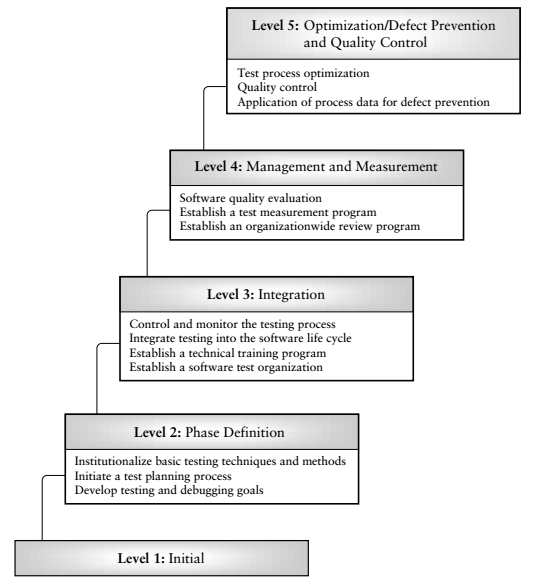
\includegraphics[scale=0.85]{img/TMMI}
    \caption{TMMi modelio brandos lygiai \cite{Burnstein:2010:PST:1965566}}
    \label{img:tmmi}
\end{figure}


\section{Eksperimentinio palyginimo rezultatai}
% tablesgenerator.com - converts calculators (e.g. excel) tables to LaTeX
\begin{table}[H]\footnotesize
  \centering
  \caption{Lentelės pavyzdys}
  {\begin{tabular}{|l|c|c|} \hline
    Algoritmas & $\bar{x}$ & $\sigma^{2}$ \\
    \hline
    Algoritmas A  & 1.6335    & 0.5584       \\
    Algoritmas B  & 1.7395    & 0.5647       \\
    \hline
  \end{tabular}}
  \label{tab:table example}
\end{table}

\end{document}
